\documentclass[11pt,a4paper]{article}
\usepackage{fontspec}
\usepackage{polyglossia}
\setdefaultlanguage{russian}
\setotherlanguage{english}
\setmainfont{Arial}
\usepackage{amsmath,amssymb,mathtools}
\usepackage{geometry}
\usepackage{graphicx}
\usepackage{booktabs,tabularx}
\usepackage{xcolor}
\usepackage{hyperref}
\usepackage{enumitem}
\usepackage{fancyhdr}
\geometry{left=22mm,right=22mm,top=22mm,bottom=22mm}
\definecolor{navy}{HTML}{17324D}
\definecolor{blue}{HTML}{2563EB}
\definecolor{soft}{HTML}{EFF6FF}
\definecolor{green}{HTML}{15803D}
\hypersetup{colorlinks=true,linkcolor=blue,urlcolor=blue}
\setlength{\parskip}{5pt}
\setlength{\parindent}{0pt}
\setlist{nosep,leftmargin=1.4em}
\pagestyle{fancy}
\fancyhf{}
\lhead{\small Модель посадки Луны-16}
\rhead{\small Конспект физики и уравнений}
\cfoot{\thepage}
\newcommand{\dd}{\mathop{}\!d}
\newcommand{\er}{\mathbf e_r}
\newcommand{\etheta}{\mathbf e_\theta}
\newcommand{\vv}{\mathbf v}
\newcommand{\uu}{\mathbf u}
\newcommand{\Tmax}{T_{\max}}
\newcommand{\Isp}{I_{\mathrm{sp}}}
\title{\textbf{\color{navy}Физическая модель посадки}\\[3pt]\large Уравнения для Луны и Mun в KSP}
\author{Рабочий конспект}
\date{}
\begin{document}
\maketitle
\vspace{-1.1cm}
\begin{center}
\fcolorbox{blue}{soft}{\parbox{0.91\linewidth}{\centering
\textbf{Главная идея.} Строим одну модель движения аппарата с переменной массой. Для расчёта на Луне и Mun оставляем уравнения одинаковыми и меняем параметры небесного тела и аппарата.}}
\end{center}

\section{1. Что именно моделируем}
Рассматриваем участок от низкой орбиты до касания поверхности. Аппарат считаем материальной точкой. На него действуют центральное тяготение выбранного тела и тяга двигателя. Атмосферу, рельеф, колебания корпуса и возмущения от других тел в первой версии не учитываем.

Это \textbf{модель посадочного манёвра}, а не модель перелёта Земля--Луна. Исторические данные «Луны-16» задают контрольные события, а полные ряды высоты и скорости мы получим из собственной симуляции KSP.

\subsection*{Система координат и обозначения}
Начало координат находится в центре небесного тела. Используем плоские полярные координаты:
\begin{itemize}
\item $r$ --- расстояние от центра тела до аппарата, м;
\item $\theta$ --- угловое положение аппарата, рад;
\item $v_r=\dot r$ --- радиальная скорость; при снижении $v_r<0$;
\item $v_\theta=r\dot\theta$ --- скорость вдоль местной касательной;
\item $R$ --- радиус тела, $h=r-R$ --- высота над поверхностью;
\item $m$ --- текущая масса аппарата, кг;
\item $T$ --- модуль тяги, Н; $T_r,T_\theta$ --- её радиальная и тангенциальная компоненты.
\end{itemize}
Положительное направление $\er$ направлено от центра наружу. Положительное направление $\etheta$ выбрано по орбитальному движению. Поэтому при торможении тангенциальная компонента тяги отрицательна.

\begin{center}
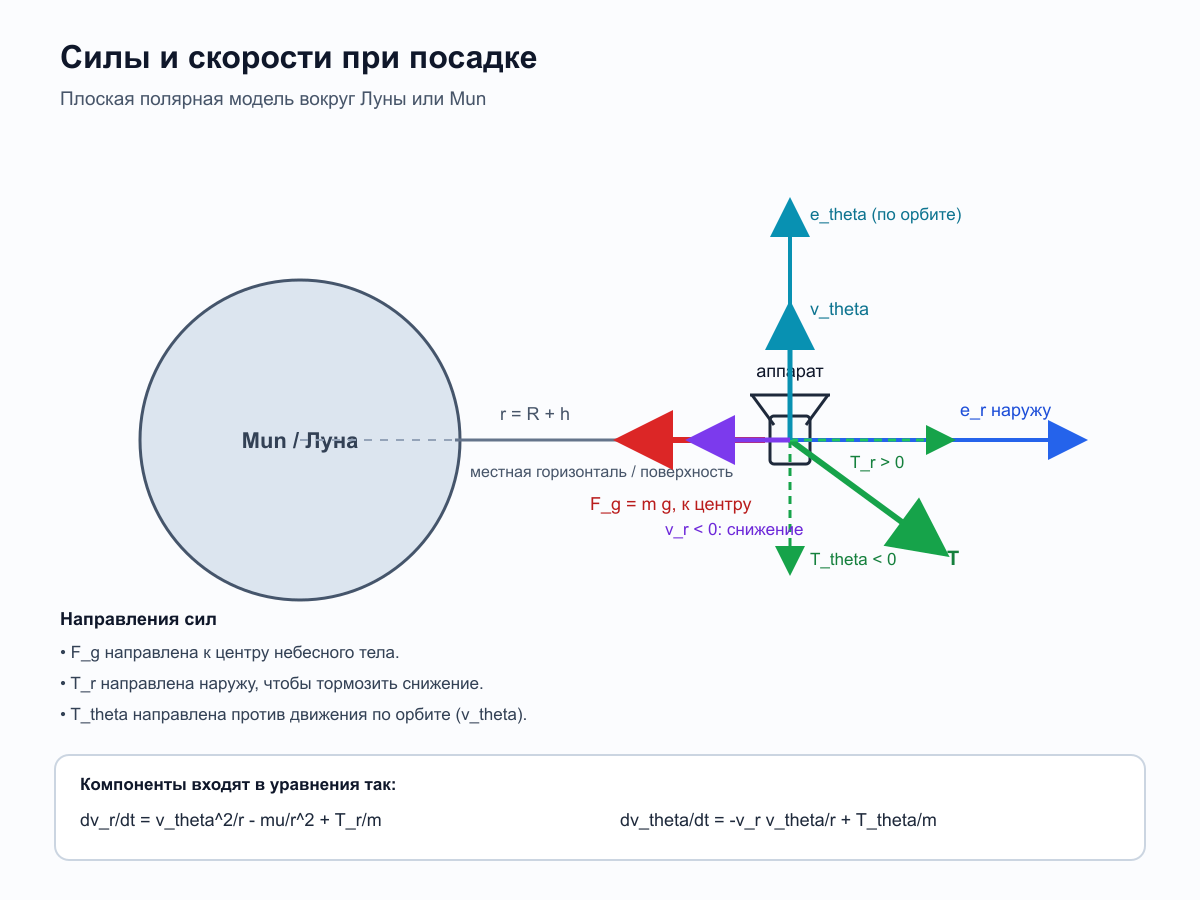
\includegraphics[width=0.94\linewidth]{images/forces.png}
\end{center}

\section{2. Силы и закон движения}
Гравитационный параметр тела:
\[
\mu=GM,
\]
где $G$ --- гравитационная постоянная, $M$ --- масса небесного тела. Сила тяготения направлена к центру:
\[
\mathbf F_g=-\frac{\mu m}{r^2}\er.
\]
Тягу раскладываем на составляющие в выбранных осях:
\[
\mathbf T=T_r\er+T_\theta\etheta.
\]
Здесь $T_r>0$ означает тягу наружу, а $T_\theta<0$ --- тягу против движения по орбите. Второй закон Ньютона для аппарата:
\[
m\frac{\dd\vv}{\dd t}=\mathbf F_g+\mathbf T.
\]
После деления на массу:
\[
\frac{\dd\vv}{\dd t}=-\frac{\mu}{r^2}\er+\frac{T_r}{m}\er+\frac{T_\theta}{m}\etheta.
\]
Удельные ускорения от двигателей равны $T_r/m$ и $T_\theta/m$. При одинаковой тяге более лёгкий аппарат ускоряется сильнее.

\section{3. Переход к полярным уравнениям}
В полярных координатах ускорение имеет радиальную и тангенциальную части:
\[
\mathbf a=(\ddot r-r\dot\theta^2)\er+(r\ddot\theta+2\dot r\dot\theta)\etheta.
\]
Связь скоростей с координатами:
\[
v_r=\dot r,\qquad v_\theta=r\dot\theta.
\]
Сравниваем компоненты ускорения с гравитацией и тягой.

\subsection*{Радиальное уравнение}
Так как $r\dot\theta^2=v_\theta^2/r$, получаем:
\[
\boxed{\dot r=v_r,\qquad
\dot v_r=\frac{v_\theta^2}{r}-\frac{\mu}{r^2}+\frac{T_r}{m}.}
\]
Слагаемое $v_\theta^2/r$ связано с движением по кривой орбите. Гравитация даёт ускорение к центру $-\mu/r^2$. Радиальная тяга может противодействовать падению.

\subsection*{Тангенциальное уравнение}
Из $v_\theta=r\dot\theta$ следует:
\[
\boxed{\dot\theta=\frac{v_\theta}{r},\qquad
\dot v_\theta=-\frac{v_rv_\theta}{r}+\frac{T_\theta}{m}.}
\]
Первое слагаемое возникает из-за изменения радиуса во время движения. Второе меняет горизонтальную орбитальную скорость. При торможении $T_\theta<0$.

\section{4. Переменная масса и уравнение Мещерского}
Ракета ускоряется, выбрасывая продукты сгорания. Удобная форма уравнения Мещерского для двигателя с известной тягой:
\[
\boxed{\dot m=-\frac{T}{\Isp g_0}},
\qquad g_0=9.80665\ \mathrm{m/s^2}.
\]
$\Isp$ измеряется в секундах. Знак минус показывает, что масса при работе двигателя убывает. Расход топлива в кг/с равен $T/(\Isp g_0)$.

Если $T$ уже является тягой двигателя, дополнительный «ракетный» член в уравнение ускорения добавлять не нужно: обмен импульсом с выбрасываемым газом уже заключён в тяге. Когда двигатель выключен, $T=0$ и $\dot m=0$.

Полезная проверка размерностей:
\[
\frac{\mathrm{N}}{\mathrm{s}\cdot\mathrm{m/s^2}}
=\frac{\mathrm{kg\,m/s^2}}{\mathrm{m/s}}
=\mathrm{kg/s}.
\]

\section{5. Полная система состояния}
Для численного расчёта удобно объединить переменные в вектор:
\[
\mathbf x(t)=
\begin{bmatrix}
r&\theta&v_r&v_\theta&m
\end{bmatrix}^{\mathsf T}.
\]
Тогда система имеет вид:
\[
\boxed{
\begin{aligned}
\dot r&=v_r,\\
\dot\theta&=\frac{v_\theta}{r},\\
\dot v_r&=\frac{v_\theta^2}{r}-\frac{\mu}{r^2}+\frac{T_r}{m},\\
\dot v_\theta&=-\frac{v_rv_\theta}{r}+\frac{T_\theta}{m},\\
\dot m&=-\frac{T}{\Isp g_0}.
\end{aligned}}
\]
Это правая часть задачи Коши $\dot{\mathbf x}=f(t,\mathbf x,\mathbf u)$ для численного интегратора. Управление $\mathbf u$ определяет тягу и её направление.

\section{6. Как задать двигатель и управление}
В простейшем случае команда throttle $q$ принимает значения от 0 до 1:
\[
T=q\Tmax,\qquad 0\le q\le1.
\]
Если двигатель не может работать ниже минимальной тяги, задают $q=0$ либо $q\in[q_{\min},1]$. Для нескольких режимов двигателя задаём отдельные $\Tmax$ и $\Isp$ на каждом режиме.

Направление тяги можно задавать компонентами $T_r,T_\theta$. Их модуль должен соответствовать выбранной тяге:
\[
T=\sqrt{T_r^2+T_\theta^2}.
\]
Альтернативно, если $\beta$ --- угол от направления «наружу» к направлению против орбитального движения, то:
\[
T_r=T\cos\beta,\qquad T_\theta=-T\sin\beta.
\]
При $\beta=0$ тяга строго наружу; при $\beta=90^\circ$ --- строго против орбитального движения. Для реального аппарата угол также ограничивается возможностью поворота двигателя или корпуса.

Автопилот позже будет выбирать $q(t)$ и $\beta(t)$ по измеряемым $h,v_r,v_\theta$. Физическая модель сама по себе не задаёт закон управления; это отдельный блок проекта.

\section{7. Этапы спуска и режимы модели}
\begin{tabularx}{\linewidth}{@{}p{0.22\linewidth}X X@{}}
\toprule
Этап & Что происходит & Модельное описание\\
\midrule
Начальное состояние & Аппарат на низкой орбите; заданы положение и скорость & Начальные условия $\mathbf x(0)$\\
Торможение & Уменьшаем орбитальную скорость тягой против движения & $T_\theta<0$, тяга включена\\
Свободный участок & Двигатель выключен & $T_r=T_\theta=0$, масса постоянна\\
Финальное снижение & Гасим радиальную скорость и уменьшаем высоту & Обычно $T_r>0$; тангенциальную скорость доводим до цели\\
Касание & Аппарат достигает поверхности & Событие $h=0$ завершает интегрирование\\
\bottomrule
\end{tabularx}

Для воспроизведения последовательности «Луны-16» этапы включения и выключения можно задать как переключения режима. Для автоматической посадки KSP автопилот может менять throttle и направление тяги непрерывно. Это разные законы управления поверх одной и той же динамики.

\section{8. Упрощённая вертикальная модель}
Для проверки знаков и расхода топлива можно временно отбросить орбитальную скорость и рассматривать только вертикальное движение. Пусть ось высоты направлена вверх, скорость $v=\dot h$:
\[
\boxed{\dot h=v,\qquad
\dot v=\frac{T}{m}-\frac{\mu}{(R+h)^2},\qquad
\dot m=-\frac{T}{\Isp g_0}.}
\]
При снижении $v<0$. Эту модель удобно отлаживать первой, но она не описывает торможение горизонтальной орбитальной скорости и потому не является полной моделью схода с орбиты.

\section{9. Начальные условия, останов интегрирования и критерии}
Интегрирование начинается с заданного состояния:
\[
\mathbf x(0)=
\begin{bmatrix}
R+h_0&\theta_0&v_{r0}&v_{\theta0}&m_0
\end{bmatrix}^{\mathsf T}.
\]
Значения $h_0,v_{r0},v_{\theta0},m_0$ берём из выбранного сценария KSP или задаём из справочной реконструкции. Начальное состояние должно соответствовать конкретному моменту перед посадочным манёвром.

Поверхностное событие:
\[
g(\mathbf x)=h=r-R=0.
\]
Интегратор останавливается при первом достижении поверхности сверху вниз. Посадка считается мягкой, если в момент контакта выполнены критерии, например:
\[
|v_r|\le v_{r,\max},\qquad |v_{\theta,\mathrm{rel}}|\le v_{\theta,\max}.
\]
В первой версии вращение тела не учитываем и используем $v_{\theta,\mathrm{rel}}\approx v_\theta$. Если учитываем вращение с угловой скоростью $\Omega$ на широте $\varphi$, скорость поверхности вдоль восточного направления равна $\Omega r\cos\varphi$, поэтому:
\[
v_{\theta,\mathrm{rel}}=v_\theta-\Omega r\cos\varphi.
\]
Это поправка для сравнения с фактической скоростью относительно грунта; включать её нужно одновременно в модели и обработке телеметрии.

\section{10. Что меняется для Луны и Mun}
Функциональная форма уравнений одна. Параметры храним отдельно:
\begin{center}
\begin{tabularx}{0.96\linewidth}{@{}lXX@{}}
\toprule
Параметр & Луна & Mun в KSP\\
\midrule
$\mu$ & $4.9028\times10^{12}\ \mathrm{m^3/s^2}$ & Получить для используемой версии игры/модов\\
$R$ & $1.7374\times10^6\ \mathrm{m}$ & Получить для Mun из KSP\\
$T_{\max},\Isp,m_0$ & Параметры выбранного аналога или справочные оценки «Луны-16» & Фактические значения собранного аппарата\\
Атмосфера & Нет & Для Mun атмосферы нет\\
\bottomrule
\end{tabularx}
\end{center}
Важно не подставлять лунную гравитацию в прогон KSP на Mun: для каждого прогона используем константы именно выбранного небесного тела. Значения для Mun зависят от установленной игры и модификаций, поэтому их следует записать из используемой конфигурации.

\section{11. Исторические контрольные точки «Луны-16»}
Опубликованные источники описывают последовательность спуска: выключение основного двигателя около $2.45$ км, свободный участок примерно $43$ с, повторное включение около $600$ м, переход на малую тягу около $20$ м и скорость касания около $4.8$ м/с. Эти значения нужны как контроль событий, а не как непрерывный временной ряд телеметрии. Точные временные ряды $h(t),v(t),m(t)$ для всей посадки в доступных публикациях не приведены.

Масса станции при посадке в источниках приводится примерно $1.88$--$1.90$ т. Для расчётов надо выбрать одно значение, указать источник и считать его исходной оценкой. Цель автопилота KSP, например касание менее $2\ \mathrm{m/s}$ по вертикали, является нашим критерием, а не фактическим результатом «Луны-16».

\subsection*{Разобранный пример: пассивный участок 2.45 км → 600 м}
Опубликованы высота выключения основного двигателя $h_0\approx2450\ \mathrm{m}$, длительность пассивного участка $t=43\ \mathrm{s}$ и высота повторного включения $h_1\approx600\ \mathrm{m}$. Это контрольные точки из описания миссии; открытая покадровая телеметрия для этого участка здесь не используется.

На пассивном участке $T=0$, поэтому масса постоянна, а для грубой оценки используем вертикальное уравнение с постоянной лунной гравитацией $g\approx\mu/R^2\approx1.624\ \mathrm{m/s^2}$. Направим скорость вниз как положительную величину $u=-v_r$. Тогда пройденное расстояние:
\[
h_0-h_1=u_0t+\frac{gt^2}{2}.
\]
Отсюда начальная скорость вниз, подразумеваемая этой упрощённой моделью:
\[
u_0=\frac{(h_0-h_1)-gt^2/2}{t}
=\frac{1850-1.624\cdot43^2/2}{43}
\approx8.1\ \mathrm{m/s}.
\]
К концу свободного падения:
\[
u_1=u_0+gt\approx8.1+1.624\cdot43\approx77.9\ \mathrm{m/s}.
\]
Это \textbf{расчётная реконструкция по опубликованным контрольным точкам}, а не считанная из бортового журнала скорость. Она показывает, как свободный участок кодируется в модели: положить $T=0$, интегрировать $\dot h=v_r$ и $\dot v_r=-\mu/(R+h)^2$, затем проверить высоту через 43 секунды.

\subsection*{Пример расхода топлива на малой тяге}
Для блока KTDU-417B опубликованы диапазон тяги $2.06$--$3.43\ \mathrm{kN}$ и $\Isp\approx252$--$254\ \mathrm{s}$. Возьмём только для оценки $T=3.00\ \mathrm{kN}$, $\Isp=253\ \mathrm{s}$ и $m\approx1880\ \mathrm{kg}$:
\[
\dot m=-\frac{3000}{253\cdot9.80665}\approx-1.21\ \mathrm{kg/s},\qquad
a_T=\frac{T}{m}\approx1.60\ \mathrm{m/s^2}.
\]
На поверхности лунная тяжесть около $1.62\ \mathrm{m/s^2}$, поэтому такая вертикальная тяга почти уравновешивает тяжесть. Это объясняет, зачем малой тяге нужен регулируемый режим: около посадки небольшая разность между тягой и весом определяет, продолжает ли аппарат снижаться или начинает тормозить вверх. Значения двигателя и массы здесь справочные; это не точный расчёт конкретного момента полёта.

\section{12. Какие графики и показатели сравнивать}
Сохраняем одинаковые по смыслу ряды для численной модели и KSP:
\[
h(t),\quad v_r(t),\quad v_{\theta,\mathrm{rel}}(t),\quad m(t),\quad T(t).
\]
Сравниваем время посадки, скорость касания, максимальное расхождение траекторий и значения на исторических контрольных высотах. Для каждого мира выполняем отдельный расчёт с его $\mu,R$ и параметрами аппарата. Исторические данные Луны не являются прямой телеметрией Mun; они проверяют правдоподобие модели и этапов.

\section{13. Список допущений первой версии}
\begin{enumerate}
\item Небесное тело сферическое, гравитация центральная: $g(r)=\mu/r^2$.
\item Движение плоское; боковые отклонения от плоскости не рассматриваются.
\item Атмосфера и аэродинамические силы отсутствуют.
\item Аппарат представлен материальной точкой; ориентационная динамика корпуса отдельно не моделируется.
\item Масса меняется только за счёт расхода топлива; сброс ступеней не моделируется.
\item Рельеф и ударная динамика опор не рассчитываются; критерии проверяются в момент контакта.
\item Вращение тела сначала исключается; при необходимости добавляется поправка на скорость поверхности.
\end{enumerate}

\section{14. Порядок ручного вывода}
\begin{enumerate}
\item Нарисовать центр тела, локальные оси $\er,\etheta$, радиус $r$, аппарат, $\vv$, $\mathbf F_g$ и компоненты тяги.
\item Записать закон Ньютона $m\dot{\vv}=\mathbf F_g+\mathbf T$ и закон изменения массы.
\item Выписать выражение для ускорения в полярных координатах.
\item Приравнять радиальную и тангенциальную компоненты и получить два уравнения скорости.
\item Добавить кинематические связи $\dot r=v_r$, $\dot\theta=v_\theta/r$ и уравнение расхода массы.
\item Проверить знаки: гравитация внутрь, тормозная радиальная тяга наружу, тормозная тангенциальная тяга против $v_\theta$.
\end{enumerate}

\section*{Источники исходных характеристик}
\begin{itemize}
\item NASA NSSDC, Moon Fact Sheet: \url{https://nssdc.gsfc.nasa.gov/planetary/factsheet/moonfact.html}
\item JPL Solar System Dynamics, параметры спутников: \url{https://ssd.jpl.nasa.gov/sats/phys_par/sep.html}
\item Журнал «Новости космонавтики», № 11, 2010, описание этапов посадки «Луны-16»: \url{https://epizodsspace.airbase.ru/bibl/nk/2010/nk2010-11.pdf}
\item НПО им. С. А. Лавочкина, «Луна-16»: \url{https://www.laspace.ru/ru/activities/archive_launch/luna-16-e-8-5/}
\item C. Schmierer, \textit{Analysis of a Hybrid Propulsion}, 2019, технические параметры двигательной установки: \url{https://elib.dlr.de/133092/1/2019%20Schmierer%20Dissertation.pdf}
\end{itemize}
\end{document}
